This problem is solved using the set of point $S$ produced by the algorithm \ref{algStaticGuard}. Based on the knowledge of this points, clearing the whole area can be done easily. It is enough to have each guard visiting once each of this points to guarantee that there is no static intruder (since the whole area will be seen). Figure \ref{dynamicPath} shows the paths for 4 vehicles cleaning an area.

The problem can then be stated as the following:

\begin{subproblem}
 Knowing the set of point $S$ and with a given number $n_{G}$ of guard, find the minimum path for each guard with the following condition:
\begin{itemize}[topsep=0pt,itemsep=0ex,partopsep=1ex,parsep=1ex]
  \item Each point has been seen once,
  \item The time to visit each point of $S$ is the smallest possible.
 \end{itemize}
This problem is quiet similar to the vehicles routing problem.
\label{subProb3}
\end{subproblem}

\subsection{Problem modelization}

The problem is modelize as the following:

\begin{enumerate}[topsep=0pt,itemsep=0ex,partopsep=1ex,parsep=1ex]
  \item Create a matrix \textbf{Cost} with $\text{\textbf{Cost}}_{i,j} = \text{Length}(P_i,P_j)$ (real path length).
  \item Index each point of $S$ from $1$ to $n_{S}$.
  \item Index each guard from $n_{S}+1$ to $ n_{S}+n_{G}$.
  \item Each permutation $\sigma$ of $\{1,\hdots,n_{S}+n_{G}\}$ is a potential solution if $\sigma$ satisfy criteria \ref{permCriteria}
  \item  We will look for the solution where the guards have the smallest path possible : $$Cost(\sigma_1) \leq Cost(\sigma_2)$$ $$\Longleftrightarrow$$
	$$\max_{k,\sigma_1}\text{PathLength}(\text{Guard}_k)\leq \max_{k,\sigma_2}\text{PathLength}(\text{Guard}_k)$$
\end{enumerate}

\begin{criteria}
 Given a set $S$ of $n_S$ points and $n_G$ guards, a permutation $\sigma$ of $\{1,\hdots,n_S+n_G\}$ is valid if each $\sigma_i \in \sigma$ has a predecessor stricly bigger than $n_S$  -- it means that each point is visited once.
 \label{permCriteria}
\end{criteria}


\subsection{Exhaustive search}

Algorithm \ref{algExhDynamic} is testing every permutation of $\{1,\hdots,n_{S}+n_{G}\}$, but rapidly check if a permutation is a real potential solution, getting rid of a maximum of them. This algorithm performed well for small value of $n_S + n_G$ (until $\approx 10$).

\begin{algorithm}
This algorithm gives a way to find the smallest path for a set of $n_{G}$ vehicle to visit a set $S = P_{1\leq i \leq n_S}$ of point.
\begin{enumerate}[topsep=0pt,itemsep=0ex,partopsep=1ex,parsep=1ex]
  \item Generate a valid permutation of $\{1,\hdots,n_{S}+n_{G}\}$.
  \item If each indices in $\{n_S +1, \hdots , nS +nG\}$ are in ascending order and if each robot visit a maximum of $\left \lceil{\frac{n_S}{n_G}}\right \rceil$  points (ceil function)
	\begin{enumerate}[topsep=0pt,itemsep=0ex,partopsep=1ex,parsep=1ex]
  \item Compute the total length represented by the permutation using the matrix \textbf{Cost}.
  \item Keep this permutation in memory if its the best so far.
  \end{enumerate}
\item While there is valid permutations go to 1.
\end{enumerate}
\qed
\label{algExhDynamic}
\end{algorithm}


\subsection{Tabu search}

Algorithm \ref{algExhDynamic} has a upper limit of $10$ since its checking every possible permutation. We need to be able to explore bigger environment -- more points to explore and/or more guards. In order to do so, we implemented a tabu--search like algorithm. Its performances are more than decent and its computational time is \emph{almost} constant, providing a solution close to the optimal one.

It is needed to understand the following notions before reading algorithm \ref{algExhDynamic}:
\begin{description}[topsep=0pt,itemsep=0ex,partopsep=1ex,parsep=1ex]
 \item[Tabu-list:] List of fixed size with a storage of the permutation already processed in the close past.
 \item[Diversification:] If the algorithm is stuck in a local minima, diversification is needed. 
To do so, we generate a random valid permutation and start our search from there.
 \item[Neighborhood:] Given a permutation $\sigma$, its neighborhood is defined has the permutations than can be reached from $\sigma$ by applying a swap of two adjacent index ($i \leftrightarrow i+1$) or a swap of 4 adjacents number ($(i,i+1) \leftrightarrow (i+2,i+3)$)
\end{description}


\begin{algorithm}
  This algorithm provide a way to find a ``close to optimal'' solution of problem \ref{subProb3} 
\begin{enumerate}[topsep=1ex,itemsep=0ex,partopsep=1ex,parsep=1ex]
   \item Generate a random valid permutation $\sigma_{best}$.
   \item Generate all the valid permutations in the \textbf{neighborhood} of $\sigma_{best}$.
   \item Foreach $\sigma_{potential}$ in this \textbf{neighborhood}
\begin{enumerate}[topsep=0pt,itemsep=0ex,partopsep=1ex,parsep=1ex]
    \item If $\sigma_{potential}$ is not in the tabu-list
    \begin{enumerate}
     \item Check if its a better solution than $\sigma_{best}$ (and eventually replace it)
     \end{enumerate}
   \end{enumerate}
     \item Add $\sigma_{best}$ to the tabu-list.
     \item If the solution has not improved since a given number of step, apply \textbf{diversification}.
   \item While the maximum of step has not been reached, go to 2. 
  \end{enumerate}
   \qed
 \label{tabuSearchAlg}
\end{algorithm}

In our case, algorithm \ref{tabuSearchAlg} has proved itself good with the following parameters:
\begin{itemize}[topsep=0pt,itemsep=0ex,partopsep=1ex,parsep=1ex]
 \item 10.000 steps
 \item Diversification after 20 steps with no improvement
 \item Tabu-list of size 100
\end{itemize}




\begin{figure}[h!t]
	\begin{center}
	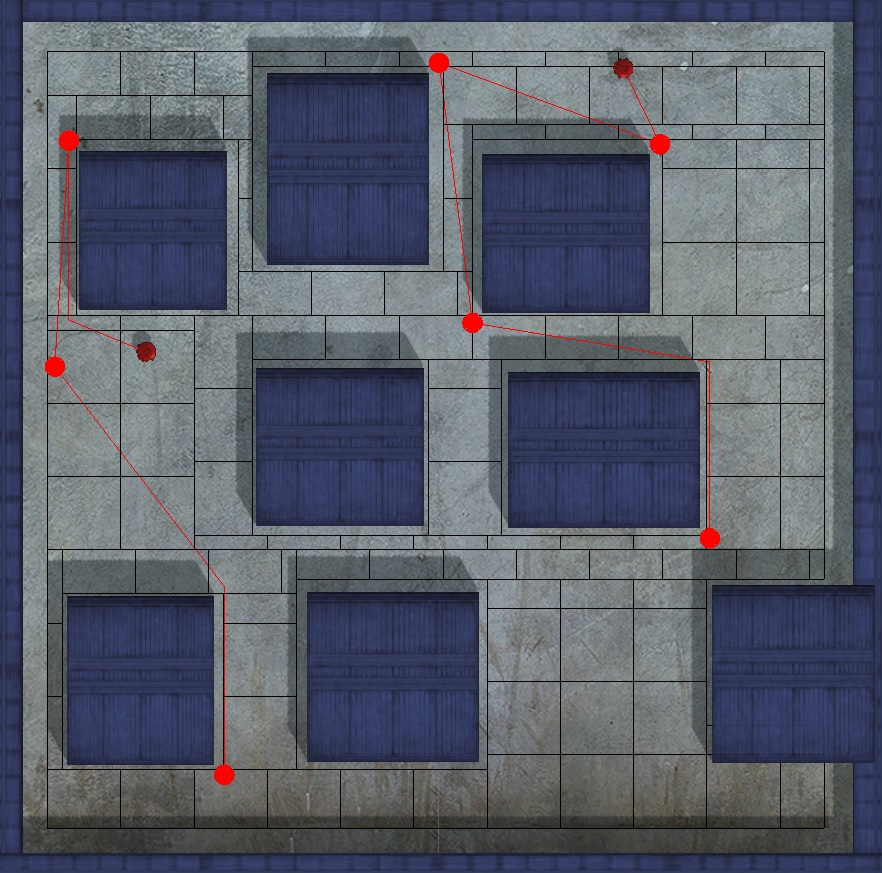
\includegraphics[width=150px]{fig/dynamicPath.jpg}
	\end{center}
	\caption{Path for $4$ vehicles (green) looking for a static intruder}
	\label{dynamicPath}
\end{figure}


